\section{Block-Encoding}
\label{sec:block-encoding}

Quantum algorithms are restricted to being composed by a series of unitary operators.
However, it is often necessary to access information about various non-unitary operators within a quantum algorithm.
``Block-Encoding" refers to a type of access model where the information regarding non-unitary operators is encoded in a labeled subspace (block) of a larger unitary operator.

If $A$ represents some $N_A \times N_A$ non-unitary operator, then a block-encoding of $A$ in matrix form is given by:
\begin{equation}
    U_A = 
    \begin{pmatrix}
    \bar{A} & * \\
    * & * 
    \end{pmatrix}
\end{equation}
where $U_A$ is a unitary operator, $\bar{A}$ is a rescaled form of $A$ such that the spectral norm ($||\bar{A}||$) is less than or equal to $1$, and matrix entries $*$ denote matrix elements that ensure $U_A$ is unitary.

The action of $U_A$ on an arbitrary quantum state ($\ket{\psi}$) with dimension $N_A$ can be defined as:
\begin{equation}
    \label{eq:general-block-encoding}
    U_A \ket{\psi} \ket{0}_{\text{anc}} = \bar{A} \ket{\psi} \ket{0}_{\text{anc}} + \beta_\psi \ket{\perp}
\end{equation}
where $\ket{}_{\text{anc}}$ is a register of block-encoding ancillae used to produce the $U_A$ and $\beta_\psi$ is a complex coefficient that normalizes the output quantum state.
The portion of the state given by $\ket{\perp}$ represents the branch of the wavefunction that is orthogonal to any state in the encoded subspace.
In the above equations, the encoded subspace of the block-encoding is chosen (without loss of generality) to be the all-zero state of the block-encoding ancillae.

It is important to note that $\beta_\psi$ is dependent on the initial state of the system register ($\ket{\psi}$).
The dependence of $\beta$ on $\ket{\psi}$ can be seen in a simple case where $\ket{\psi}$ is an eigenstate of $\bar{A}$.
If $\ket{\lambda_k}$ is an eigenstate of $\bar{A}$ with eigenvalue $k$, then Eq. \ref{eq:general-block-encoding} leads to:
\begin{equation}
    U_A \ket{\lambda_k} \ket{0}_{\text{anc}} = k \ket{\lambda_k} \ket{0}_{\text{anc}} + \sqrt{1 - |k|^2} \ket{\perp}
\end{equation}
where $\sqrt{1 - |k|^2}$ is clearly dependent upon the eigenvalue associated with the eigenstate.

One way to interpret the action of the block-encoding is that it produces a probabilistic application of $\bar{A}$.
After the block-encoding is applied, if a measurement of the block-encoding ancillae results in all of those qubits being in the zero state, then $\bar{A}$ has been applied to the quantum state.
The probability for this measurement result to occur is given by $\text{P}(0) = ||\bar{A} \ket{\psi}||^2$.

The rescaling factor ($\lambda$) of a block-encoding is given by:
\begin{equation}
    A = \lambda \bar{A}
\end{equation}
This rescaling factor can have important implications in the cost of quantum algorithms. 
Smaller rescaling factors generally lead to more efficient algorithms though the exact impact on the cost is algorithm-dependent.
For example, the success probability of applying $\bar{A}$ as described above decreases as $\lambda$ increases.
If the block-encoding is used to construct a quantum walk operator \cite{low2019hamiltonian, poulin2018quantum} and used in Quantum Phase Estimation \cite{poulin2018quantum, babbush2018encoding, lee2021even}, then the output eigenvalue estimates are scaled by the rescaling factor which will affect both the error and the precision of the estimate.

In the following subsections, we will describe some commonly used frameworks for constructing block-encodings of different operators.
In particular, we discuss both the Sparse-Oracle and Linear Combination of Unitaries (LCU) frameworks for generating block-encodings.
Then we discuss methods to combine block-encodings of operators to produce block-encodings for a linear combination of operators or a product of operators.

\subsection{Sparse-Oracle Framework}
\label{subsec:sparse-be}

The Sparse-Oracle framework \cite{berry2009black, childs2009universal, berry2015hamiltonian,berry2015simulating, low2017optimal,childs2017quantum,gilyen2019quantum} assumes the presence of oracles that provide both the location and the values of the nonzero matrix elements.
When an operator is sparse within some known basis, the Sparse-Oracle framework can build off of this structure to heavily reduce the cost of the block-encoding construction.

Let $A$ be a matrix with a maximum of $s$ nonzero entries in a single row and each matrix element of $A$ has magnitude $\leq 1$.
Let $A_{ij}$ be the matrix element in the $i^\text{th}$ row and the $j^\text{th}$ column.

Lin et. al \cite{lin2022lecture} defines three oracles ($D_s$, $O_A$, and $O_c$) to produce a Sparse-Oracle block-encoding.
The ``diffusion operator'' $(D_s)$ is defined by:
\begin{equation}
    \label{eq:diffusion}
    D_s \ket{0^{\log_2{s}}} = \frac{1}{\sqrt{s}} \sum_{l=0}^{s-1} \ket{l}
\end{equation}
Where $s$ is increased to the nearest power of $2$ by treating some zero-valued elements as nonzero.
This oracle can be implemented by a tensor product of Hadamards: $H^{\otimes \log_2{s}}$.

The ``column oracle'' ($O_c$) is defined by: 
\begin{equation}
    \label{eq:column-oracle}
    O_c \ket{j} \ket{l} = \ket{j}\ket{c(j, l)}
\end{equation}
where $c(j, l)$ is a function that returns the row-index of the $l^\text{th}$ nonzero matrix element in the $j^\text{th}$ column.

Lastly, the ``value oracle'' ($O_A$) is defined by:
\begin{equation}
    \label{eq:value-oracle}
    O_A \ket{0} \ket{j}\ket{i} = \big( A_{ij} \ket{0}  + \beta_{ij} \ket{1} \big) \ket{j}\ket{i}
\end{equation}
where $\beta_{ij} \equiv \sqrt{1 - |A_{ij}|^2}$.

With these three oracles, a block-encoding for $A$ is given by:
\begin{equation}
    \label{eq:so-be}
    U_A = D_s O_c O_A D_s
\end{equation}
with a rescaling factor of:
\begin{equation}
    \label{eq:rescaling-so}
    \lambda_\text{SO} = 2^n \max_{ij} {|A_{ij}|} 
\end{equation}
A simple proof that $U_A$ block-encodes $A$ is given in Camps et. al \cite{camps2024explicit}.

The factor of $\max_{ij} {|A_{ij}|}$ in the rescaling factor (Eq. \ref{eq:rescaling-so}) comes from the constraint that all elements of $A$ have magnitude at most $1$.
The factor of $2^n$ comes from the sparsity of $A$.
If $s$ is not a power of two, then this factor can be reduced to $s$ by replacing the ``diffusion operator" with the generalized \textit{Uniform State Preparation} (USP) protocol which is discussed in more detail in Appendix \ref{sec:usp}.
Implementing USP typically requires more nontrivial operations than the diffusion operator, so a trade-off exists between reducing the rescaling factor and reducing the time complexity.

A framework for compiling quantum circuits that implement these oracles for general matrices ($D_s$, $O_A$, and $O_c$) is given in \cite{camps2024explicit, camps2022fable} and Sparse-Oracle block-encodings for particular systems have been explored in several works \cite{camps2022fable, liu2024efficient, sanavio2024explicit}.

\subsection{Linear Combination of Unitaries Framework}
\label{subsec:lcu}

An alternative framework proposed by Childs et. al \cite{childs2012hamiltonian} called Linear Combination of Unitaries (LCU) is \textit{specifically} designed for generating block-encodings of operators that can be written in the following form:
\begin{equation}
    \label{eq:lcu}
    A = \sum_{l=0}^{L-1} \alpha_l U_l
\end{equation}
where $\alpha_l$ are positive, real-valued coefficients and each $U_l$ is a unitary operator.
For terms with negative or imaginary coefficients, the sign and imaginary phase can be absorbed into the operator: $-i \alpha_l U_l = \alpha_l (-i U_l)$.
Likewise, a term with a complex coefficient can be treated as two distinct terms, each with a real coefficient.

To generate an LCU block-encoding, two oracles, \textit{Prepare} and \textit{Select}, are required. The \textit{Prepare} oracle serves a similar role to the $O_A$ oracle in that it loads the coefficients or the values of the matrix elements onto the quantum computer.
The action of the \textit{Prepare} oracle is to map the all-zero state of an ancilla register to a particular superposition state where the squared amplitudes of the computational basis states are weighted to encode the coefficients of the terms in the operator:
\begin{equation}
    \label{eq:prep-state}
    \textbf{Prepare}\text{:} \ket{0^{\otimes \lceil \log_2 L \rceil}}_\text{index} \rightarrow \sum_{l=0}^{L-1} \sqrt{| \alpha_l | / \lambda} \ket{l}_\text{index}
\end{equation}
where $\lambda$ is given by:
\begin{equation}
    \label{eq:lambda-lcu}
    \lambda_\text{LCU} = \sum_{l=0}^{L-1} | \alpha_l |
\end{equation}
The block-encoding ancillae register is often referred to as the \textit{index register} as the computational basis states of this register $(\ket{l})$ index the $L$ terms in Eq. \ref{eq:lcu}.

The desired action of the \textit{Select} oracle is to apply the unitary $(U_l)$ onto the system register when the index regsiter is in the computation basis state $\ket{l}$:
\begin{equation}
    \label{eq:select}
    \textbf{Select}\text{:} 
    \begin{cases} 
        \text{Apply $U_l$ on $\ket{\psi}$} & \text{when $\ket{\text{index}}$ is $\ket{l}$ and $l < L$} \\
        \text{Undefined} & \text{Otherwise} \\
    \end{cases}
\end{equation}
and the action of the \textit{Select} oracle is not strictly defined for the computational basis states outside of the range $[0, L)$.

With these two oracles, a block-encoding for $A$ is given by:
\begin{equation}
    \label{eq:lcu-be}
    U_A = (\textbf{Prepare}^\dagger) (\textbf{Select}) (\textbf{Prepare})
\end{equation}
with an overall rescaling factor of $\lambda_\text{LCU}$ (Eq. \ref{eq:lambda-lcu}).
A simple proof that $U_A$ block-encodes $A$ is given in Section 7.3 of Lin et. al \cite{lin2022lecture}.

A block-encoding for $A$ could also be generated using the Sparse-Oracle framework, but would result in a rescaling factor of $\lambda_\text{SO} = 2^{\lceil \log_2L \rceil} \max_l |\alpha_l|$.
A simple proof that $\lambda_\text{LCU} \leq \lambda_\text{SO}$ is given in Appendix \ref{sec:proof-of-rescaling-factors}.

\subsubsection{Implementing \textbf{Prepare}}

The matrix representation for a valid implementation of the \textit{Prepare} oracle in the computational basis is given by:
\begin{equation}
    \text{Prepare} = \begin{bmatrix}
        \sqrt{|\alpha_0| / \lambda_\text{LCU}} & * & ... & * \\
        \sqrt{|\alpha_1| / \lambda_\text{LCU}} & * & ... & * \\
        \vdots & \vdots & \ddots & \vdots \\
        \sqrt{|\alpha_{L-1} |/ \lambda_\text{LCU}} & * & ... & * \\
    \end{bmatrix}
\end{equation}
From this definition, it is clear that there are infinitely many unitaries that implement the $\textit{Prepare}$ oracle since only the first column of the operator is fixed.

The Grover-Rudolph algorithm \cite{grover2002creating} gives a formulaic routine to generate quantum circuits that implement the $\textit{Prepare}$ oracle.
The cost of implementing Grover-Rudolph scales exponentially with the number of qubits in the register it acts upon.
However, the size of the index register is logarithmic in the number of terms ($L$), therefore the number of operations required to implement Grover-Rudolph is linear in $L$.

For operators that have structure among the coefficients of the terms, implementations of $\textit{Prepare}$ can be constructed that leverage this structure to reduce the number of operations required to implement the oracle.
In certain cases, this can drastically reduce the cost such as is done for the Fermi-Hubbard model in \cite{babbush2018encoding}.

\subsubsection{Implementing \textbf{Select}}

% \begin{figure}[h]
%     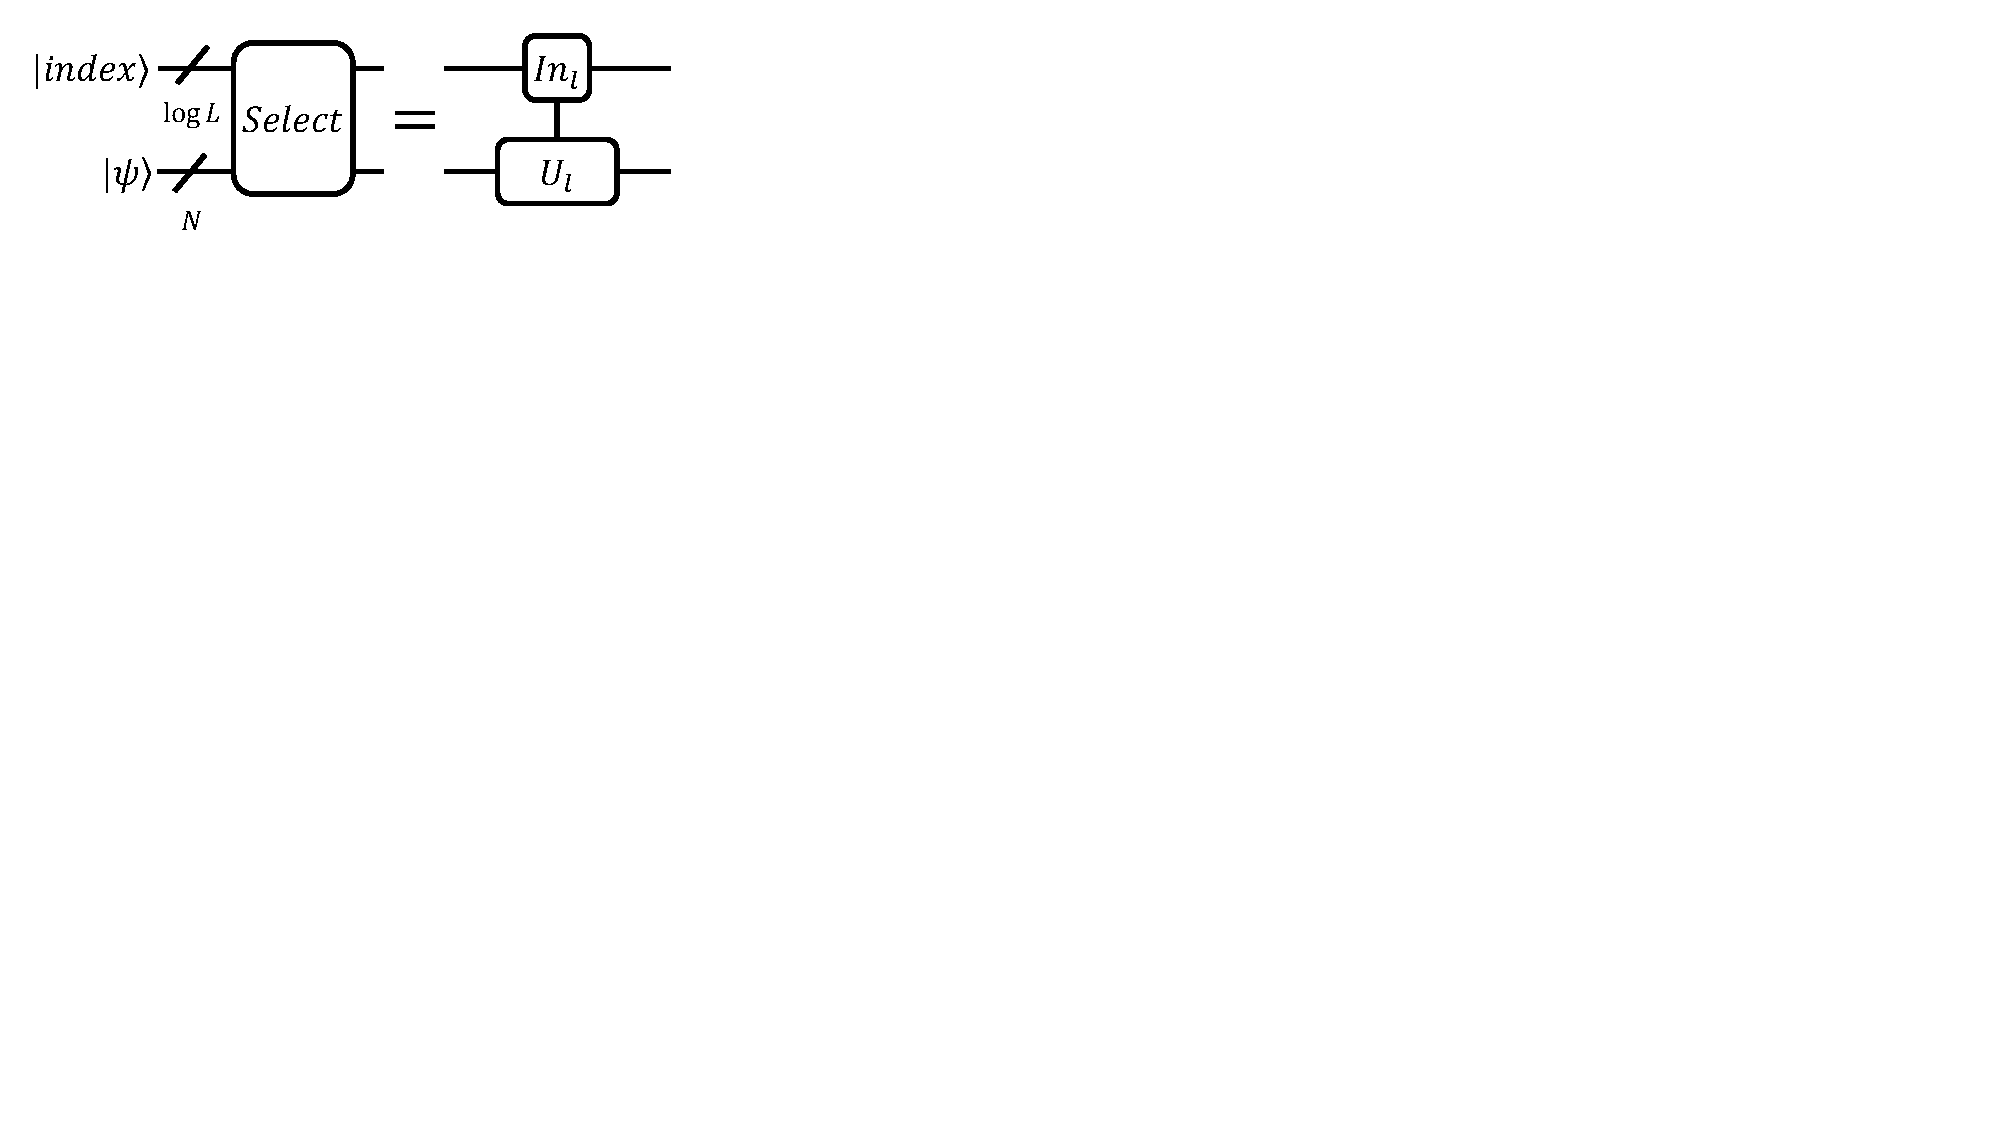
\includegraphics[width=6cm]{figures/select-lcu.pdf}
%     \caption{
%         \textbf{LCU \textit{Select} Oracle Implementation}
%         The \textit{Select} oracle applies the $l^\text{th}$ unitary in Eq. \ref{eq:lcu} onto the system when the index register is in the computational basis state $\ket{l}$
%         This series of operations be achieved using a set of uniformly controlled operations (right subfigure).
%     }
%     \label{fig:unstructured-select}
% \end{figure}

Without any assumptions on the structure of $A$, the \textit{Select} oracle can be implemented by the operator:
\begin{equation}
    \label{eq:select-naive}
    U_\text{Select} = \sum_{l=0}^{L-1} \ket{l}\bra{l} \otimes U_l + \sum_{l>L} \ket{l}\bra{l} \otimes \mathds{1}
\end{equation}

In this above form, $U_\text{Select}$ is restricted to apply the identity operator for computational basis states of the index register outside of the range $[0, L-1)$.
However, if this constraint is relaxed or if there is structure in the description of the operator, then a more efficient implementation of $\textit{Select}$ can be constructed as is done in \cite{babbush2018encoding}.  

As an aside, if the implementation of the \textit{Select} oracle is self-inverse, then the LCU block-encoding is also self-inverse.
This structure makes LCU block-encodings particularly well-suited for being applied in algorithms based on Qubitization \cite{low2019hamiltonian}.
The construction for \textit{Select} in Eq. \ref{eq:select-naive} is naturally self-inverse if the unitaries themselves are self-inverse, which is true when the operator is decomposed in the Pauli basis.

\subsection{Block-Encoding Linear Combinations of Non-Unitary Operators}
\label{subsec:lco}

% LCU block-encodings provide better rescaling factors, yet there are clearly parallels between the $O_A$ oracle and the \textit{Prepare} oracle, as well as the $O_c$ oracle and the \textit{Select} oracle.
A natural question to ask is if the structure of an LCU block-encoding can be generalized to a linear combination of non-unitary operators:
\begin{equation}
    \label{eq:lco}
    A = \sum_{l=0}^{L-1} \alpha_l O_l
\end{equation}
where the $O_l$ are operators and we again restrict the coefficients $\alpha_l$ to be positive and real-valued for simplicity.

Let the set of unitary operators $\{U_l\}$ represent block-encodings of the operators $O_l$:
\begin{equation}
    \label{eq:applying-operator}
    U_l \ket{\psi}\ket{0}_\text{anc} = \bar{O}_l \ket{\psi} \ket{0}_\text{anc} + \beta_{\psi, l} \ket{\perp}
\end{equation}
where each block-encoding uses the same encoded subspace and has a rescaling factor $\lambda_l$ such that $\lambda_l \bar{O}_l = O_l$.
Additionally, let the operator $\Tilde{A}$ be defined by the linear combination of the block-encoding unitaries:
\begin{equation}
    \Tilde{A} = \sum_{l} \Tilde{\alpha_l} U_l \hspace{1em} \Tilde{\alpha_l} = \frac{\alpha_l \lambda_l}{\max_{l^\prime}{\lambda_{l^\prime}}}
\end{equation} 
Then an LCU block-encoding of $\Tilde{A}$ will also give a block-encoding of $A$ with an overall rescaling factor of:
\begin{equation}
    \lambda = \sum_{l=0}^{L-1} |\alpha_l \lambda_l|
\end{equation}

\ws{Is this paragraph helpful/necessary or should it be removed?}
The fact that $U_{\Tilde{A}}$ block-encodes $A$ can be seen from the linearity of the operators themselves:
\begin{equation}
    U_{\Tilde{A}} = 
    \begin{pmatrix}
    \bar{\Tilde{A}} & * \\
    * & * 
    \end{pmatrix} \propto
    \sum_{l}
    \begin{pmatrix}
    \Tilde{\alpha_l} U_l & * \\
    * & * 
    \end{pmatrix} =
    \sum_{l}
    \begin{pmatrix}
    \begin{pmatrix}
        \alpha_l O_l & * \\
        * & * 
    \end{pmatrix} & * \\
    * & * 
    \end{pmatrix} 
\end{equation}
It is clear from this form that the block-encodings $\{U_l\}$ must all have the same encoded subspace as they would otherwise not yield the desired linear combination in the encoded subspace of $U_{\Tilde{A}}$.
It is also worth noting that the block-encodings $\{U_l\}$ may all use the same block-encoding ancillae as long as the implementation of the \textit{Select} oracle ensures that the ancillae begin in the all-zero state in the subspace in which each block-encoding unitary is applied.

As noted in prior works \cite{berry2015simulating, childs2017quantum, gilyen2019quantum, lin2022lecture, jennings2023efficient}, this process can be thought of as producing a linear combination matrices on the quantum computer.
Alternatively, it may be enlightening to consider an LCU block-encoding as a apecial case of an LCO block-encoding wherein the operators in the linear combination are all unitary.
In this work, we will refer to a block-encoding of this form as a Linear Combination of Operators (LCO).

\subsection{Block-Encoding Products of Non-Uniatry Operators}
\label{subsec:be-products}

Likewise, it is natural to ask if a block-encoding for a product of operators can be easily produced, assuming access to block-encodings for the individual operators.
As noted by Gilyén et. al \ref{gilyen2019quantum}, a block-encoding for a product of operators can be constructed by the product of the block-encodings of the individual operators.

Let $A$ represent a product of operators $B$ and $C$:
\begin{equation}
    \label{eq:product}
    A = BC
\end{equation}
with block-encodings $U_B$ and $U_C$.
Then, the product of $U_B$ and $U_C$ results in a block-encoding of $A$:
\begin{equation}
    \begin{split}
        U_B U_C \ket{\psi} \ket{0}_\text{anc,C}\ket{0}_\text{anc,B} &= U_B \big(\bar{C} \ket{\psi} \ket{0}_\text{anc,C} + \beta_{\psi, C} \ket{\perp}\big)\ket{0}_\text{anc,B} \\
        &= \bar{B} \bar{C} \ket{\psi} \ket{0}_\text{anc,C} \ket{0}_\text{anc,B} + \beta_{\psi, C, B} \ket{\perp}
    \end{split}
\end{equation}
with an overall rescaling factor of $\lambda = \lambda_B \lambda_C$.

It is important to note that in general the block-encodings for the individual operators require separate block-encoding ancillae.
This constraint ensures that each block-encoding unitary acts on an ancilla register beginning in the all-zero state to adhere to the form of Eq. \ref{eq:general-block-encoding}.